\chapter{GPU implementation}

This chapter guides the reader through the implementation of the Mahalanobis-based hierarchical clustering analysis. First, we describe the algorithm and the high level look on the implementation. Then, we thoroughly describe the most important functions.

\section{The algorithm choice}

The first chapter introduced three views on implementation of hierarchical clustering. To decide which one to choose, we need to take into an account two conditions. First, the algorithm should not require a quadratic space complexity as it must be able to process rather large datasets. Second, the algorithm should exhibit some parallelism opportunities; otherwise massive GPU parallel properties will be to no use.  We describe the mentioned algorithms according to this conditions:
\begin{description}

\item[HCA with dissimilarity matrix] satisfies the first condition if the dissimilarity matrix will not be held in the memory. The second condition is satisfied as each matrix field can be computed independently, exposing great parallelism opportunity. 

\item[HCA with the nearest neighbor array] has needed sub-quadratic space complexity by definition. On the other hand, it provides less space for a parallelism as the algorithm need not to compute whole dissimilarity matrix as~in~the~previous algorithm. However, large dataset sizes may compensate for this disadvantage. 

\item[HCA with priority queues] is unusable as it does not satisfy the first condition. Moreover, operation over priority queues (insert, delete and min) are not of a parallel nature and may create a bottleneck in the computation.

\end{description}

For this thesis we chose to implement HCA with the nearest neighbor array. It promises better time complexity than the HCA with dissimilarity matrix which can come to a great use when clustering big datasets. In addition, we utilized the~advantages of priority queues by defining a constant that declares the~number of~closest neighbors assigned to each cluster.

Additionally, we chose to implement the CMD variant of the Mahalanobis distance to fully exhibit GPU parallel properties.

\subsection{Apriori clusters}

When cluster sizes reach the Mahalanobis threshold, a MHCA algorithm starts to form elliptic clusters. However, until then, a simple euclidean distance is used. This is an important stage of the algorithm as an improper initial clustering can decrease the overall clustering result. Hence, a simple hierarchical euclidean clustering can be unsatisfactory.

To solve this problem, we implemented an additional feature called the \emph{apriori clusters}. 

\begin{defn}[Apriori clusters]
	Suppose a dataset $\mathcal{D}$, a HCA algorithm $\mathcal{A}$ and a~partitioning of  $\mathcal{D}$ into non-empty subsets $\mathcal{D}_1,\dots,\mathcal{D}_k$. If following conditions hold:
	\begin{enumerate}
		\item $\mathcal{A}$ performs clustering of each subset separately. Meaning that clusters from different subsets can not be merged.
		\item When each subset is clustered into the only cluster, $\mathcal{A}$ clusters the resulting clusters as if they were in one subset.
	\end{enumerate}
	then we call the subsets $\mathcal{D}_1,\dots,\mathcal{D}_k$ \emph{apriori clusters} of $\mathcal{A}$.
	\label{def03:apriori}
\end{defn}

The intended usage of the feature is that the apriori clusters are created from a dataset using non-hierarchical clustering algorithm such as \emph{k-means} --- an algorithm that is capable of creating better initial clusters that the MHCA algorithm.

With this feature, the MHCA algorithm is guided by the apriori clusters to~create the corresponding merged clusters. They are usually of a small size that just reached the Mahalanobis threshold and can fully exhibit the MHCA properties. Overall, we suppose that apriori clusters can lessen the probability of~an~error during the early stage of the algorithm.

\section{Generic interface to clustering algorithms}

The chosen algorithm is implemented in the main class of the program --- \texttt{gmhc}\footnote{An abrevation for GPU Mahalanobis-based Hierarchical Clustering}. It inherits from an abstract template class \texttt{hierarchical\_clustering}.
This template provides key data fields and methods for a hierarchical clustering algorithm (see list.~\ref{lst03:hc}): 

\begin{description}
	\item[\texttt{initialize()}] sets the fields of the class. A templated field \texttt{points} is an array of dataset objects --- points. They are expected to be of a floating-point numeric type. Fields \texttt{point\_dim} and \texttt{points\_size} state a point dimensionality and a total number of points in the array. Hence, each \texttt{point\_dim} consecutive array elements represent one point and the total array size is~$\texttt{point\_dim}*\texttt{points\_size}$ elements.
	
	\item[\texttt{run()}] initiates the clustering. It returns a vector of \texttt{pasgnd\_t} structures --- pairs that contain \emph{assignments} and a \emph{distance} --- the IDs of merged clusters and~the~distance between them. Each point from the input array is assigned an~unique consecutive ID starting from $0$. When two clusters are merged, the new cluster is assigned the next available unique ID. The process of merging is then stored in the returning vector. Hence, the vector completely describes the whole clustering process.
	
	\item[\texttt{free()}] deallocates all acquired resources.
\end{description}

\begin{lstlisting}[caption={A summary of \texttt{hierarchical\_clustering} header file.},label={lst03:hc}]
using csize_t = uint32_t;
using asgn_t = csize_t;
using pasgn_t = std::pair<asgn_t, asgn_t>;
template <typename T>
using pasgnd_t = std::pair<pasgn_t, T>;

template <typename T>
class hierarchical_clustering
{
protected:
	const T* points;
	csize_t points_size;
	csize_t point_dim;
public:
	virtual void initialize(...);
	virtual std::vector<pasgnd_t<T>> run() = 0;
	virtual void free() = 0;
};
\end{lstlisting}

\section{Mahalanobis clustering implementation}

The class \texttt{gmhc} is the main entrypoint of the whole MHCA algorithm. It inherits from \texttt{hierarchical\_clustering<float>} template specialization, which means that the algorithm expects dataset objects to be single-precision points of~a~specified dimension. The class communicates
with a GPU; hence, it holds structures used by the device.

It contains an array of \texttt{clustering\_context\_t} objects. Each of them holds the context of a specific part of the dataset and is able to perform a clustering on~it.

\subsection{Initialization}

Initialization happens in the \texttt{initialize} method. Due to the initialization of device and host structures, this stage must be treated with importance.
The class overloads \texttt{initialize} method so that it sets three additional fields:
\begin{itemize}
	\item \texttt{mahalanobis\_threshold} indicates the threshold in the \emph{Altered general distance} (see def.~\ref{def01:alt}).
	
	\item\texttt{apriori\_assignments}  is an array of assignments that splits \texttt{points} into \emph{apriori clusters}. This is an optional field of the \texttt{initialize} method.
	
	\item \texttt{validator} is an optional field used for testing purposes.
\end{itemize}

Next follows the main responsibility of the \texttt{initialize} method --- device and host data allocation and initialization. They are \emph{point}, \emph{assignment}, \emph{centroid}, \emph{inverse covariance}, \emph{neighbor} and \emph{status arrays}.

\begin{defn}[Point array]
	Suppose a dataset $\mathcal{D}$ that contains objects represented by $k$-di\-men\-si\-onal ponts. We define \emph{point array} $\mathcal{P}$ as an array that contains consecutive sequence of all objects in $\mathcal{D}$.
	\label{def03:point}
\end{defn}

\begin{defn}[Assignment array]
	Suppose a partitioning of a point array $\mathcal{P}$ into~clusters $c_1,\dots,c_k$ where each cluster $c_i$ is defined by its unique ID $id_i$ and a set of indices $I_i$ that state which points from $\mathcal{P}$ belong to the cluster. The array of length $|\mathcal{P}|$ is the \emph{assignments array} $\mathcal{A}$ when for each cluster $c_i$ the following equation holds:
	$${\forall j \in I_i : \mathcal{A}_j = id_i}$$
	\label{def03:assign}
\end{defn}

\begin{defn}[Cluster-based arrays]
	Given a dataset $\mathcal{D}$, its clusters $c_1,\dots,c_k$, a Mahalanobis threshold $T_M$ and a positive number $m$, we define the following \emph{cluster-based arrays}:
	\begin{itemize}
		\item the \emph{centroid array} $\mathcal{C}$ as an array that contains centroids of all $k$ clusters,
		\item the \emph{inverse covariance array} $\mathcal{I}$ as an array that contains inverse covariance matrices of all clusters that reached $T_M$,
		\item the \emph{neighbor array} $\mathcal{N}$ as an array that contains indices and distances to the~$m$~closest neighbors of all $k$ clusters,
		\item the \emph{status array} $\mathcal{S}$ as an array that contains sizes and unique ids of all $k$~clusters.
	\end{itemize}
	\label{def03:tuple}
\end{defn}


All but the status array are device arrays. Device data are used within kernels while host data control the flow of run kernels.  

To indicates a location of a cluster data distributed among the cluster-based arrays, we define their \emph{indexing structure}: 

\begin{defn}[Indexing structure]
	Having a dataset $\mathcal{D}$, its $k$ clusters and a corresponding cluster-based array tuple $(\mathcal{C},\mathcal{I},\mathcal{N},\mathcal{S})$, we define the \emph{indexing structure} $\mathcal{Q}$ that determines the order of the cluster-related data in this arrays.
	\label{def03:index}
\end{defn}

For each cluster, the indexing structure is able to retrieve an index to~the~clus\-ter-related arrays pointing to its data. The most importantly, data about a specific cluster resides under the same index within all cluster-related arrays.



\subsection{Clustering}
The clustering algorithm resides in the method \texttt{run}. This method utilizes the~array of \texttt{clustering\_context\_t} objects --- instances of a \emph{clustering context} --- that divide the dataset according to the provided apriori clusters.

\begin{defn}[Clustering context]
	Given a dataset $\mathcal{D}$, its point array $\mathcal{P}$, assignment array $\mathcal{A}$ and cluster-based array tuple $(\mathcal{C},\mathcal{I},\mathcal{N},\mathcal{S})$ with its indexing structure $\mathcal{Q}$, we define the \emph{clustering context} of $\mathcal{D}' \subset \mathcal{D}$ as a tuple $(\mathcal{P'},\mathcal{A'},\mathcal{C'},\mathcal{I'},\mathcal{N'},\mathcal{S'},\mathcal{Q}')$. In the tuple, each array is a sub-array of the corresponding array of $\mathcal{D}$. Each sub-array contains data of points and clusters created within $\mathcal{D}'$. $\mathcal{Q}'$ describes the order of the sub-arrays.
	\label{def03:context}
\end{defn}

 If \texttt{apriori\_assignments} are present, each element of the array serves as the~clustering context for a corresponding apriori cluster and holds methods for its further clustering. Hence, it will be further called the \emph{context array}. 

In addition to that, the method \texttt{run} uses one special clustering context called the \emph{final context}. If apriori clusters are present (and the clustering context array is non-empty), it is unset and serves as a context that will host all the apriori cluster results for the final clustering. If there are no apriori clusers, the final context is set and contains the whole dataset.

We divide the whole clustering algorithm into a top level \emph{apriori clustering} and a low level \emph{context clustering}.

\begin{description}
	\item[Apriori clustering] handles a separate clustering of apriori clusters, merging their results into one clustering context and performing the final clustering (see alg.~\ref{alg03:apriori}).
	
	The algorithm iterates over each apriori cluster from the context array. It performs its clustering using context clustering method and the result is inserted into the final context. Either when all apriori clusters are merged or when there are none at all, the final context with the remaining clusters is clustered and the list of assignment pairs is returned.
	
	Before any context begins the clustering, its closest neighbor array has to~be initialized. It is done by the kernels \texttt{neighbors}.
	
	
	\begin{algorithm}
		\caption{Apriori clustering}
		\label{alg03:apriori}
		\begin{algorithmic}[1]
			\Procedure{apriori}{context array $\mathcal{T}$, the final context $ctx_f$}
			\ForAll{$ctx \in \mathcal{T}\cup ctx_f$} \Comment{iterate over apriori clusters and the final context}
			\State initialize the closest neighbor array of $ctx$ 
			\While{$ctx$ has not the only cluster}
			\State perform context clustering of $cxt$ for the closest pair $(i,j)$ and their distance $d$
			\State store $((i,j),d)$ into the returning list
			\EndWhile
			\State $ctx_f \gets ctx_f \cup ctx$ \Comment{assign merged cluster into the final context}
			\EndFor
			\State \textbf{return} list of merged clusters
			\EndProcedure
		\end{algorithmic}
	\end{algorithm}

	\item[Context clustering] performs one iteration of clustering within the specified context --- a merge of two closest clusters (see alg.~\ref{alg03:context}). First, it goes through the neighbor array of the context and finds the closest pair of clusters (kernel \texttt{neighbor\_min}). At that moment, there are two clusters to be removed and one new cluster to be created. Hence, cluster-based arrays of~the~context need to be updated accordingly.
	
	The remainder of the algorithm sets data for the new cluster. First, $\mathcal{A}$ is recomputed to correctly show that points of the former two clusters now belong to the new one (kernel \texttt{merge\_clusters}). Then the centroid of~the~new cluster is computed and stored into $\mathcal{C}$ (kernel \texttt{centroid}) and status array is updated as well. Last, if the new cluster reaches the Mahalanobis threshold, its inverse covariance matrix is computed and stored into $\mathcal{I}$ (kernels \texttt{compute\_icov}). 
	
	The final statement of the method checks the whole $\mathcal{N}$  according to the one created and two deleted clusters and updates is when needed (kernels \texttt{update\_neighbors}).
	
	\begin{algorithm}
	\caption{Context clustering}
	\label{alg03:context}
	\begin{algorithmic}[1]
		\Procedure{context}{$\mathcal{A},\mathcal{C},\mathcal{I},\mathcal{N},\mathcal{S},\mathcal{Q}$}
		\State retrieve the clostest pair $(i,j)$ and distance $d$ from $\mathcal{N}$
		\State initialize an unique $id$ of the new cluster $c$
		\State update $\mathcal{Q}$ and retrieve new index $idx$ for $c$
		\State reorder data in $(\mathcal{C},\mathcal{I},\mathcal{N},\mathcal{S})$
		\State update $\mathcal{A}$
		\State $\mathcal{C}_{idx} \gets$ compute the centroid of $c$
		\State $\mathcal{S}_{idx} \gets \{|c|, id\}$
		\If{$|c| \ge \texttt{mahalanobis\_threshold}$}
		\State $\mathcal{I}_{idx} \gets$ compute the inverse covariance matrix of $c$
		\EndIf
		\State update $\mathcal{N}$
		\State \textbf{return} $((i,j),d)$
		\EndProcedure
	\end{algorithmic}
\end{algorithm}

\end{description}


\subsection{Data order}

This section will describe the actual process of reorganizing the cluster-related arrays provided that cluster pair $(i,j)$ is to be merged.

This is achieved with a help of a \texttt{cluster\_bound\_t} structure --- an implementation of the indexing structure $\mathcal{Q}$. It is a rather simple structure that describes how the cluster-based arrays organize their data. The structure distinguishes two parts of the arrays. The first part contains data about clusters whose size have not reached the Mahalanobis threshold while the second part stores data of remaining clusters. Hence, it contains a pair of indices indicating beginnings of the two parts and another pair describing the size of the parts. We will respectively call them \emph{Euclidean} and \emph{Mahalanobis array parts}. Note, the structure is uniform for each cluster-based array; meaning that a different array data about the same cluster resides on the same index.

When a cluster pair $(i,j)$ is to be merged, the indexing structure first recognizes the part of an array where the indices $i$, $j$ belong. Hence, it identifies the places of arrays that are no longer valid. It gets rid of the places in the two particular ways:
\begin{itemize}
	\item Assign the invalid place as the place for the new cluster.
	\item Moves the end data of the corresponding part to the invalid place.
\end{itemize}
The reason why we organize the data in such way is to maintain continuously distributed data (see fig.~\ref{fig03:data_order}). This data distribution serves a great help for running device kernels.

\begin{figure}\centering
	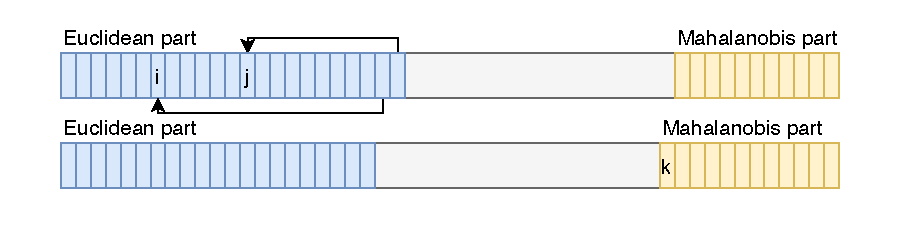
\includegraphics[width=\textwidth]{img/data}
	\caption{An example of the data distribution in a cluster-related array. Two clusters of non-Mahalanobis size with their indices $i$, $j$ are being merged into a Mahalanobis-sized cluster on index $k$.}
	\label{fig03:data_order}
\end{figure}

\begin{rem}
	Naturally, there are other ways to maintain continuously distributed data within arrays. We can move the data in such way that the new cluster will always reside in the beginning of the corresponding part of an array. This approach could decrease the complexity of several kernels. On the other hand, this requires at most linear time to move the data instead of a constant time.
\end{rem}

\section{Kernels}

Kernels handle the computation critical parts of the algorithm. They are divided into several groups:

\begin{itemize}
	\item \emph{Clusters merging} updates an assignment array to reflect a merging of two clusters.
	\item \emph{Centroid computation} goes through an assignment array and computes the centroid of the newly formed cluster. 
	\item \emph{Inverse covariance matrix computation} is a set of kernels that computes the~inverse of the covariance matrix of newly formed clusters that reached the Mahalanobis threshold. 
	\item \emph{Minimum retrieval} iterates over a neighbor array to find the closest clusters.
	\item \emph{Neighbor array update} updates a neighbor array structure with respect to the newly created cluster.
\end{itemize}

Each kernel group reads and modifies a different data array and works in a~various time complexity. Hence, to complete the kernel summary, we provide this information in the tab.~\ref{tab03:kernels}. The following sections will describe each kernel group in more detail.

 \begin{table}
 	\centering
 	\begin{tabular}{lccccc}
 		\toprule
 		\textbf{Kernel group}                  & \mc{3}{\textbf{Read arrays}} & \textbf{Write arrays}  & \textbf{Complexity} \\ \midrule
 		\textbf{Clusters merging}              &     &   $\mathcal{A}$     &    &     $\mathcal{A}$      &       $O(n)$        \\\\
 		\textbf{Centroid computation}          &        $\mathcal{A}$  &   &$\mathcal{P}$       &  $\mathcal{C}$  &   $O(n)$\\\\
 		\textbf{Inverse covariance}\\
 		\textbf{matrix computation}            &    \pulrad{$\mathcal{A}$} &    \pulrad{$\mathcal{P}$} & \pulrad{$\mathcal{C}$}        &     \pulrad{$\mathcal{I}$}                 &       \pulrad{$O(n)$} \\\\
 		\textbf{Minimum retrieval}             &     &   $\mathcal{N}$            &&                     &       $O(c)$        \\\\
 		\textbf{Neighbor array update}         &    $\mathcal{C}$&    $\mathcal{I}$ & $\mathcal{N}$        &     $\mathcal{N}$      &      $O(c^2)$       \\ \bottomrule
 	\end{tabular}
 	\caption{The summary of the kernel groups ($n$ is a number of points in a clustering context; $c$ is a number of clusters in a clustering context).}
 	\label{tab03:kernels}
 \end{table}

\subsection{Clusters merging}


The kernel \texttt{merge\_clusters} is responsible for a clusters merging. As an input, it takes an assignment array $\mathcal{A}$, a pair of old cluster IDs (of merged clusters) and a new ID (of a new cluster). It goes through the array in the \emph{grid-stride loop} and replaces any of the old IDs with the new ID.

\begin{defn}
	A \emph{grid-stride loop} iterates over all threads in the grid until the desired number of iterations is hit. This kind of loop contrasts with the premise that a kernel grid has enough threads for the computation and does not have to iterate over the same threads multiple times (which is not always the case). 
	\label{def03:grid-stride}
\end{defn}

\subsection{Centroid computation}

Kernel \texttt{centroid} computes the centroid of a cluster with a specified $id$. According to the $id$, the kernel filters a point array $\mathcal{P}$ using an assignment array $\mathcal{A}$ to~find the involved points.

Each thread maintains its local array that stores the sum of the points that belong to the cluster. 

First, a grid-stride loop is performed over $\mathcal{P}$. If a point belongs to the cluster (determined using $\mathcal{A}$ and $id$), the thread aggregates it in the sum array. 

After the loop ends, \emph{shared memory} and \emph{warp shuffle instructions} are utilized to reduce the sum arrays of all block threads into one array (we will call this the \emph{block reduction}).

Each block reduced array is then divided by the cluster size and stored into $\mathcal{C}$ using the \emph{atomic add instruction}. 

\subsection{Inverse covariance matrix computation}


To compute inverse covariance matrix of a cluster with an $id$, multiple kernels are run from the host method \texttt{compute\_icov}. 

First, the covariance matrix of the cluster has to be computed via kernels \texttt{covariance} and \texttt{finish\_covariance}. 

Then, the \emph{CUBLAS}\footnote{CUDA implementation of BLAS library} library is used to invert the covariance matrix. If the~matrix can not be inverted (due to the singular property) the inverse is set to the identity. 

Last, a special transformation is performed on the inverse covariance matrix and the result is stored to $\mathcal{I}$ via the \texttt{store\_icovariance} kernel.

\subsubsection{Covariance matrix computation}

Kernel \texttt{covariance} computes the upper triangular covariance matrix of the cluster multiplied by the cluster size. 

To achieve a linear complexity in the number of points, we use the centroid $C$ of the cluster (it is already computed by the previous kernel). Before the kernel starts, $C$ is copied to the \emph{constant memory} so all threads can use it.

At the kernel start, each thread uniformly selects a part of the \emph{shared memory} as its intermediate upper-triangulate covariance matrix; more threads can share the same part, so atomic access is necessary.

Then, a grid-stride loop over $\mathcal{P}$ with an $id$ filtering follows. If a point belongs to the cluster, a thread subtracts it by $C$; we will denote the subtraction result with $S$. After that, each element $i$ of $S$ is separately multiplied with the element $j \ge i$ and atomically added to the corresponding place of the intermediate covariance matrix of the thread. The equation \ref{eq03:cov} describes the process. There, $\textbf{X}$ denotes the discrete random variable of the x-coordinate of all cluster points, $C_x$ denotes the x-coordinate of $C$ and $\mathbf{S_x}$ denotes discrete random variable $\mathbf{X}-C_x$.

\begin{equation}
\begin{split}
n\cov(\mathbf{X},\mathbf{Y}) &= n\mathbf{E}[(\mathbf{X}-\mathbf{E}(\mathbf{X}))(\mathbf{Y}-\mathbf{E}(\mathbf{Y}))] = n\mathbf{E}[(\mathbf{X}-C_x)(\mathbf{Y}-C_y)] \\ &= n\mathbf{E}[(\mathbf{S_x})(\mathbf{S_y})] = n\frac{1}{n}\sum_{i=1}^{n}{\mathbf{S}_{\mathbf{x}}^{i}\mathbf{S}_{\mathbf{y}}^{i}} = \sum_{i=1}^{n}{\mathbf{S}_{\mathbf{x}}^{i}\mathbf{S}_{\mathbf{y}}^{i}}
\end{split}
\label{eq03:cov}
\end{equation}

After the loop, a \emph{block sum reduction} is performed and the resulting covariances are stored to a \emph{global memory} via the \emph{atomic add instruction}.

\subsubsection{Finishing covariance matrix}
Immediately next follows the kernel \texttt{finish\_covariance}. It takes the result of~the previous kernel as an input, it divides the matrix by cluster size and transforms it to a square matrix for the inversion operation.

We could incorporate the division operation into the previous kernel. However, it would be needed to be done by each thread performing the atomic operation. Here, each element is divided just once.

\subsubsection{Storing inverse covariance matrix}
After the inversion done by the CUBLAS subroutine \texttt{cublasSmatinvBatched}, the kernel \texttt{store\_icovariance} performs the following actions with its result:
\begin{enumerate}
	\item Transforms the matrix to the upper triangulate variant.
	\item Multiplies the non-diagonal elements of the matrix by a factor $2$.
	\item Stores the transformed matrix into $\mathcal{I}$.
\end{enumerate}

The first step is performed to get rid of redundant information and to save space as the $\mathcal{I}$ array has the greatest space complexity among the cluster-based arrays.

The second step is an optimization for the computation of the Mahalanobis distance equation (see eq. \ref{eq01:maha}). We can allow this optimization as the distance is a \emph{quadratic form} that can be simplified as shown in equation \ref{eq03:form}.

\begin{equation}
\T{\mathbf{x}}\mathbf{M}\mathbf{x} = \sum_{i=1}^{n}\sum_{j=1}^{n}{m_{ij}x_ix_j} = \sum_{i=1}^{n}{m_{ii}x_i^2} + \sum_{i=1}^{n}\sum_{j>i}^{n}{2m_{ij}x_ix_j}
\label{eq03:form}
\end{equation}


\begin{rem}
The overall time complexity of the \texttt{compute\_icov} function is $O(n)$ as~for each kernel it needs to iterate over all points in a clustering context. We omitted complexity of computing a point covariance ($O(dim^2)$) and a matrix inversion ($O(dim^3)$) as the size of the point dimension is negligible compared to~the~size of the clustering context.
\end{rem}

\subsection{Minimum retrieval}

The kernel \texttt{neighbor\_min} finds the closest neighbor among all the neighbors in~the neighbor array $\mathcal{N}$.

The loop over $\mathcal{N}$ is performed block-stride as the grid must consist of just one block. That is because there is no grid synchronization in CUDA; meaning that threads can be synchronized only within the same block. In this task, we need to synchronize all involved threads.

Each thread iterates through the loop and stores its local closest neighbors (their distances and indices).

After the loop ends, the block threads perform reduction operation achieving the globally closest neighbors.

\subsection{Neighbor array update}


The kernels \texttt{update\_neighbors} is a set of five kernels where each of them takes an important part in updating the neighbor array $\mathcal{N}$.

First, the invalidated places have to be recognized by the kernel \texttt{update}. Next, two kernels \texttt{neighbors\_u} and \texttt{neighbors\_mat\_u} are run to update the~array --- the first one updates the Euclidean part while the second kernel updates the~Mahalanobis part. Then, the reduction kernel \texttt{reduce\_u} is called that takes reduces intermediate results of the previous two kernels. Last, the kernel \texttt{neighbors\_new} performs a special update of $\mathcal{N}$ for the newly created clusters.

In the apriori clustering, another kernel set is mentioned ---  \texttt{neighbors}. It is used for the initialization of $\mathcal{N}$; hence, it is a modification of the currently described kernels. There, the \texttt{update} and \texttt{neighbors\_new} kernels are ignored as all elements of the array have to be updated and none of them is created. The~notation of kernel names suggests that kernels suffixed with \texttt{\_u} has a suffix-less variant that processes all elements.

\subsubsection{Kernel \texttt{update}}
This kernel checks the validity of neighbors of each cluster via a grid-stride loop. The check consists of these steps:
\begin{itemize}
	\item If the neighbor index belongs to a cluster that was merged, remove the neighbor.
	\item If the neighbor index belongs to a cluster that was moved during an array reorder, change the index accordingly.
\end{itemize} 
When no neighbors are present, the particular cluster is marked for the update. The index of the cluster is stored in the \emph{update array} $\mathcal{U}$. It is divided into two parts --- same as for the other cluster-related arrays. 

$\mathcal{U}$ to contain continuous indices of update-ready clusters, threads synchronize over the \emph{global memory} variable indicating the next available location of $\mathcal{U}$. The variable is manipuled by threads using the \emph{atomic add instruction}.

\subsubsection{Kernel \texttt{neighbor\_u}}

This kernel takes care of updating clusters whose size have not reached the Mahalanobis threshold (we call them \emph{Euclidean clusters} for simplicity). For that reason, the kernel takes $\mathcal{C}$ as an input to compute distances --- and find the closest neighbors --- and $\mathcal{U}$ to target clusters for the computation.

The first loop is not run in parallel, rather it is fully performed by all threads as it loops through $\mathcal{U}$. When cluster $c$ is selected to update, all threads contribute to the computation of its closest neighbors.

Next, a grid-stride loop over other Euclidean clusters follows. Each thread takes care of one cluster at a time, computes its distance with $c$ and updates its local closest neighbors of $c$.

Then, a block reduction follows. The block-local closest neighbors of $c$ are created. As there is no block synchronization, each block store its result in the~intermediate neighbor array $\mathcal{N}'$ ready for a further reduction.

When all clusters from $\mathcal{U}$ are visited, the kernel ends.

\begin{rem}
	As the Altered general distance function is symmetric, there is no need to compute distance between all clusters and a cluster $c$ that needs to be updated. We only need to compute distances of clusters with their indices greater than the~index of $c$. If we follow this invariant throughout the algorithm, we can safely ignore the clusters of lower index in the computation as during \emph{theirs} computation the cluster $c$ was already involved. This does not hold for newly created clusters. They need to be measured against all the remaining clusters to~hold the invariant (the kernel \texttt{neighbors\_new}).
\end{rem}

\subsubsection{Kernel \texttt{neighbor\_mat\_u}} This kernel shows similarities with the previous kernel. The main distinction is that it updates clusters that reached the Mahalanobis threshold (\emph{Mahalanobis kernels}, for simplicity) instead of those that did not. We created the separate kernel hoping to utilize the GPU more and to achieve a better performance.

In addition to $\mathcal{C}$, the kernel takes $\mathcal{I}$ as an input as well. The access to the inverse covariance matrices is vital as they are involved in a distance computation of Mahalanobis clusters. 

Same as in the previous kernel, the first loop is performed by all threads, then followed by a grid-stride loop. 

However, one \emph{warp} takes care of one cluster at a time in the grid-stride loop. Warp threads cooperate together in the matrix-vector multiplications as the Mahalanobis distance function is now involved. The previous kernel need not to~perform such a task for computing the distance. Hence, only one thread is assigned the job there.

Last, the kernel performs the same reduction as in the previous kernel and stores the block-local intermediate results into $\mathcal{N}'$.

\begin{rem}
	The invariant of distance computation holds in this kernel as well. However, when a Mahalanobis cluster $c$ needs to be updated, distances between $c$ and \emph{all} Euclidean clusters must be also computed regardless the index. This is a~trade-off for having Euclidean and Mahalanobis clusters divided from themselves. However, the majority of Euclidean clusters tend to merge themselves early in the clustering.
\end{rem}

\subsubsection{Kernel \texttt{reduce\_u}} This is a helper kernel that reduces intermediate results of updated clusters in~$\mathcal{N}'$ into the neighbor array $\mathcal{N}$. For each updated cluster, there is as much closest neighbor entries as there were blocks in a grid of previous kernels. As this may be a big nuber, one \emph{warp} cooperates in the reduction of the entries for one updated cluster.

\subsubsection{Kernel \texttt{neighbor\_new}} The last kernel updates $\mathcal{N}$ in the means of the newly created cluster $c$. It computes the remainder of the distances (between $c$ and clusters of lower indices) to satisfy the mentioned invariant. Hence, this kernel moves this responsibility from the kernels \texttt{neighbor\_u} and \texttt{neighbor\_mat\_u} to simplify them and process the special measures faster. The kernel is called after the reduction kernel as it operates directly with $\mathcal{N}$. 

\begin{rem}
	The time complexity of the \texttt{update\_neighbors} kernels is $O(c^2)$, where $c$ denotes the number of clusters in a clustering context. This is due to the~kernels that compute the closest neighbors. In the worst case, neighbors of~each cluster need to be recomputed resulting in the mentioned time complexity. However, this is rarely the case. More often, the number of update-needed clusters resides in a yet unpredictable but reasonable scope. Hence, when we denote the number of clusters needed to be updated as $u$, we can start reasoning about the more precise time complexity $O(uc)$.
\end{rem}
